%!TEX root = ../../super_main.tex
\section{Initial Thoughts}

The \ct was in an unstable state and could not even compile when this group inherited it. The \ct does not conform to many user experience design principles and crashes on a regular basis. This section describes the most conspicuous design problems and  bugs with the \ct as it was inherited. A screenshot of the \ct, as it looked once we brought it to a compilable state, can be seen in \figref{fig:category_tool_old}. The reader is invited to reference \figref{fig:category_tool_old} while reading this section.

\begin{figure}[!htbp]
    \centering
    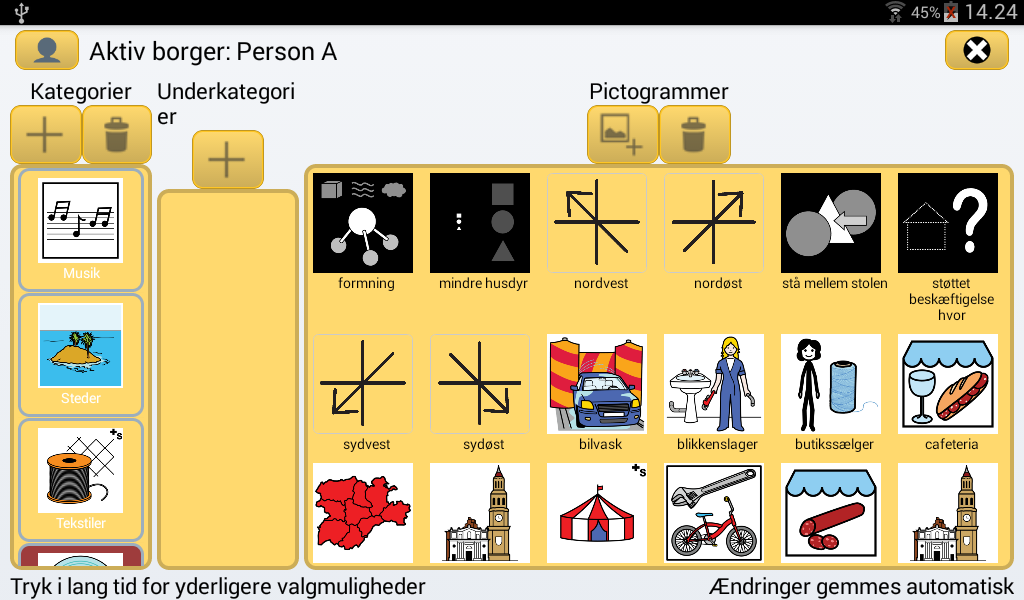
\includegraphics[width=\textwidth]{sprint_two/initial_category_tool}
    \caption{Old \ct}
    \label{fig:category_tool_old}
\end{figure}

\subsection{Interaction Design}

There is too much functionality on the same single screen in the current state of the \ct. Creation and modification of categories, sub-categories, adding and removing pictograms from categories are all done on the same screen which leaves little screen estate for each functionality.
\\\\
\todo[inline]{TODO DONE START - NIKLAS}
\todo{Try to reduce pop-up}
There are multiple contextual pop-ups throughout the application, for instance when creating a new category. The main problem with the amount of pop-ups is that the can be displayed on top of each other, for instance when the user neglects to provide a name when creating a new category. This is not a very good practice good practice and can be confusing for the user.
\\\\
Another problem with the pop-ups is that they create an overlay on top of the remaining background, but this overlay does not disappear when the Android software or hardware back buttons are pressed. This can be very confusing since this is one of the normal ways of dismissing such pop-ups.
\todo[inline]{TODO DONE END - NIKLAS}

\subsubsection{Buttons}

The \ct includes non standardized buttons of different sizes and shapes. Buttons with square icons have different rectangular shapes. Some of the buttons are too small and can be difficult to hit. There is no margin between buttons which makes it easy to misclick grouped buttons. The different buttons and widgets in the \ct are not aligned very well. There are a couple of different contextual buttons that only appear once pictograms or categories are selected. 

\subsubsection{Android Design Guidelines}

In previous versions of Android design guidelines they encouraged developers to use long press actions to open contextual menus. The guidelines have changed and now advice to exclusively use long press actions for multiple selection in lists. Long press in the \ct is currently used to show a contextual menu for categories where it is possible to change the title, color, and icon of the category and to copy it. It is currently not possible to perform multiple selection of pictograms \parencite{android_guidelines_longpress}.

\subsubsection{Selection}

When using the \ct, you are able to ``select'' different categories in order to perform some action on them (for instance deleting it). However, there are no visual cues of selection anywhere in the \ct. It is not possible to determine the currently selected category from the list of categories. This is a problem for the contextual delete button for categories. The contextual delete button for categories deletes the currently selected category but the only way to determine the current category is from the pictograms displayed to the right.

\subsection{Crashes}

The application crashes, due to unhandled out of memory errors, when there are too many pictograms in a category and the user scrolls too far down in the list. The application crashes because the application uses all of its memory on storing images that represent the pictograms in the category. 

\subsection{Explanatory Text}

There is cluttering explanatory text in the bottom of the screen which does not really help. The purpose of this explanatory text was to reveal ``hidden'' features in the application, such as telling the user to long press certain items for a contextual menu to appear, which is also against the Android Guidelines \parencite{android_guidelines_longpress}.
